\documentclass[11pt,a4paper]{article}
\newcommand{\guideshort}{Beginner quickstart}
% Shared typesetting for the two source-grounded VPE teaching guides.
\usepackage[a4paper,margin=23mm,headheight=15pt]{geometry}
\usepackage{fontspec}
\setmainfont{Liberation Serif}
\setsansfont{Liberation Sans}
\setmonofont{Liberation Mono}
\usepackage{xcolor,graphicx,booktabs,tabularx,longtable,array}
\usepackage{listings,hyperref,tikz}
\usetikzlibrary{arrows.meta,positioning}
\definecolor{vveblue}{HTML}{174A70}
\definecolor{vvelight}{HTML}{F1F5F8}
\definecolor{vvegreen}{HTML}{266547}
\hypersetup{colorlinks=true,linkcolor=vveblue,urlcolor=vveblue,
  pdfauthor={Vienna Physics Engine},pdfsubject={Source-grounded beginner teaching edition}}
\setlength{\parindent}{0pt}
\setlength{\parskip}{6pt plus 1pt}
\setlength{\emergencystretch}{3em}
\sloppy
\renewcommand{\arraystretch}{1.18}
\makeatletter
\def\ps@vve{%
  \def\@oddhead{\small\sffamily Vienna Physics Engine\hfil\guideshort}%
  \let\@evenhead\@oddhead
  \def\@oddfoot{\small\sffamily Teaching edition / 16 October 2026\hfil\thepage}%
  \let\@evenfoot\@oddfoot}
\makeatother
\pagestyle{vve}
\lstdefinestyle{vvecpp}{language=C++,basicstyle=\ttfamily\small,
  keywordstyle=\color{vveblue}\bfseries,commentstyle=\color{vvegreen},
  stringstyle=\color{vvegreen},backgroundcolor=\color{vvelight},
  breaklines=true,breakatwhitespace=false,columns=fullflexible,
  keepspaces=true,showstringspaces=false,tabsize=4,
  frame=single,rulecolor=\color{vvelight},framesep=6pt,
  xleftmargin=6pt,xrightmargin=6pt,aboveskip=8pt,belowskip=8pt,
  morekeywords={import,requires,concept,constexpr,consteval,nodiscard}}
\lstset{style=vvecpp}
\newcommand{\api}[1]{{\ttfamily\small\detokenize{#1}}}
\newcommand{\source}[1]{\par\smallskip{\raggedright\footnotesize\sffamily\color{vveblue}Source: \nolinkurl{#1}.\par}}
\newcommand{\lesson}[1]{\clearpage\section{#1}}
\newenvironment{remember}{\begin{quote}\small\textbf{Remember. }}{\end{quote}}
\newenvironment{tryit}{\begin{quote}\small\textbf{Try it. }}{\end{quote}}
\newcommand{\guidecover}[3]{%
 \begin{titlepage}\sffamily\color{vveblue}
 {\large Vienna Physics Engine\par}\vspace{20mm}
 {\Huge\bfseries #1\par}\vspace{8mm}
 {\Large #2\par}\vspace{12mm}
 \color{black}{\large #3\par}\vfill
 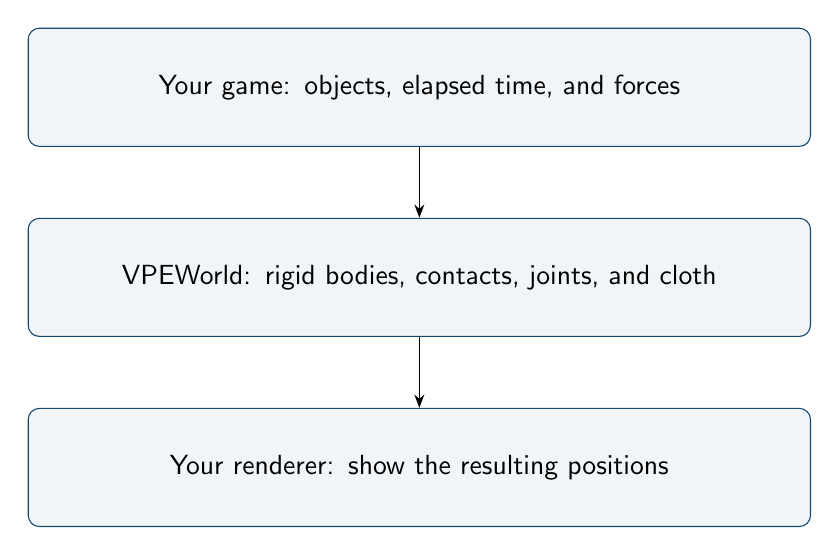
\begin{tikzpicture}[node distance=9mm,every node/.style={draw=vveblue,rounded corners,fill=vvelight,text width=0.8\linewidth,align=center,minimum height=15mm,font=\sffamily}]
 \node (game) {Your game: objects, elapsed time, and forces};
 \node (engine) [below=of game] {VPEWorld: rigid bodies, contacts, joints, and cloth};
 \node (result) [below=of engine] {Your renderer: show the resulting positions};
 \draw[-{Stealth}] (game)--(engine);
 \draw[-{Stealth}] (engine)--(result);
 \end{tikzpicture}\vfill
 {\normalsize Updated 16 October 2026\par}
 {\small Source baseline: debf892.\par}
 {\small Complete examples are checked against this source; excerpts state their context.\par}
 \end{titlepage}}

\hypersetup{pdftitle={Vienna Physics Engine - Beginner quickstart}}
\begin{document}
\guidecover{Beginner quickstart}{Your first physics objects, without a graphics setup}{A short, practical guide. Start with a falling cube, then learn how time, ownership, callbacks and cloth fit together.}
\tableofcontents
\lesson{Start here}
VPE means Vienna Physics Engine. It calculates movement and collisions. It does not open a window or draw a picture. Your game supplies objects and elapsed time; VPE gives back positions and rotations. You can learn it with a console program before connecting a renderer.

You need basic C++: variables, functions, a loop and a little familiarity with classes. A pointer stores an address. A \api{std::shared_ptr} keeps an object alive while someone still holds a copy of that pointer. Later pages explain where this matters.

The first exercise creates a cube three metres above the floor. It applies gravity, advances about two seconds and checks the final height. There is no model file, texture, Vulkan setup or VVE dependency in this exercise.

Read this guide in order for the first run. The full manual explains the same ideas more slowly, then covers collisions, joints, cloth, the solver and game integration.

\begin{remember}The public C++ module is \api{VEPhysicsEngine}. The namespace is \api{vpe}. These names are different from the repository name.\end{remember}
\lesson{Build a small console project}
Install a C++23 compiler with named module support, CMake 3.28 or newer and Ninja. On Linux the project selects Clang 18 when available and uses libc++; its development packages must be installed too. Use the repository build instructions for platform prerequisites. The standalone physics build does not need the Vulkan SDK.

Create a folder beside \api{ViennaPhysicsEngine}. Put the next page's complete program in \api{main.cpp}. Put this in \api{CMakeLists.txt}:\begin{lstlisting}
cmake_minimum_required(VERSION 3.28)
project(FirstPhysics LANGUAGES CXX)
set(CMAKE_CXX_EXTENSIONS OFF)
set(VPE_BUILD_EXAMPLES OFF CACHE BOOL "" FORCE)
set(VPE_BUILD_TESTS ON CACHE BOOL "" FORCE)
# This game folder is beside ViennaPhysicsEngine.
add_subdirectory(../ViennaPhysicsEngine vpe-build)
add_executable(first_physics main.cpp)
target_link_libraries(first_physics PRIVATE
    ViennaPhysicsEngine::ViennaPhysicsEngine)
\end{lstlisting}
On Linux with Clang 18, run these commands from your new folder:\begin{lstlisting}
cmake -S . -B build -G Ninja -DCMAKE_BUILD_TYPE=Release \
    -DCMAKE_CXX_COMPILER=clang++-18
cmake --build build
ctest --test-dir build/vpe-build --output-on-failure
\end{lstlisting}
On Windows, use a Developer PowerShell and omit the Clang compiler option so CMake uses the supported Microsoft toolchain. On macOS, select the module compiler described in the platform README. Select the compiler during the first configuration of a fresh build directory.

CMake compiles the module before its users and links the library. A plain compiler command for only \api{main.cpp} cannot arrange that dependency by itself. Find your \api{first_physics} executable in the generated build folder; the exact suffix is platform dependent.

To build the repository's own standalone checks instead, use \api{./build_linux.sh release --without-vve}, \api{./build_macos.sh release --without-vve}, or \api{.\build_windows.cmd release --without-vve}. These create a separate standalone build. Run CTest in the directory printed by the script.
\source{CMakeLists.txt; build_linux.sh; build_macos.sh; build_windows.cmd}
\lesson{A complete falling cube}
% doc-example: vpe_falling_cube
\begin{lstlisting}
#include <cmath>
#include <iostream>
#include <memory>
import VEPhysicsEngine;

int main() {
    using W = vpe::VPEWorld;
    W world;
    int owner = 1; // A stable address used as an identity.
    auto body = std::make_shared<W::Body>(
        &world, "cube", &owner, &W::g_cube,
        glmvec3{1, 1, 1}, glmvec3{0, 3, 0},
        glmquat{1, 0, 0, 0}, glmvec3{0}, glmvec3{0},
        1.0_real, 0.0_real, 0.6_real);
    W::Force gravity;
    gravity.m_accelW = {0, world.c_gravity, 0};
    body->setForce(0, std::move(gravity));
    world.addBody(body);
    const auto start = body->m_positionW.y;
    for (int frame = 0; frame < 120; ++frame)
        world.tick(1.0 / 60.0);
    const auto y = body->m_positionW.y;
    const bool ok = std::isfinite(y) && y < start
                 && y > 0.4_real && y < 0.7_real;
    std::cout << "falling_cube ok=" << ok << " y=" << y << '\n';
    world.clear(); // Owner and world are still alive here.
    return ok ? 0 : 1;
}
\end{lstlisting}
Expected result: \api{ok=1} and a height near 0.5. The cube is one metre tall and its position is its centre, so it rests about half a metre above the floor. A small collision margin explains the small offset. Exit code 0 means the check passed.
\lesson{Understand the cube one choice at a time}
\api{W world} creates the simulation. The world has a built-in horizontal floor at y = 0. The floor does not need a visible object. Positive y points up. The number passed to \api{tick} is seconds, so \api{1.0 / 60.0} is one sixtieth of a second.

\api{W::g_cube} is a ready-made convex collision shape. A convex shape has no inward dents. The scale gives the box dimensions; \api{glmvec3{1,1,1}} makes a unit cube. The next vector is its centre position. \api{glmquat{1,0,0,0}} is an identity rotation, meaning no turn. Do not use four zeroes for that rotation.

The two following vectors are linear velocity and angular velocity. Both start at zero. Linear velocity is metres per second; angular velocity is radians per second. The last numbers are inverse mass, restitution and friction. Inverse mass is 1 divided by mass: 1 means a one-kilogram body; 0 means an immovable body. Restitution controls bounce. Friction resists sliding.

Rigid bodies do not receive gravity automatically. The \api{Force} sets an acceleration in world space. The \api{setForce} ID is your chosen number; using it again replaces the same force. Forces stay active until removed. The loop advances time; \api{clear} removes bodies while their owner addresses still exist.

\begin{tryit}Change the initial height from 3 to 5. Then change inverse mass from 1 to 0. Predict which body falls before you run it. Restore inverse mass before continuing.\end{tryit}
\lesson{Keep owners and shapes alive}
The owner pointer is an identity label for your game object. VPE does not own or delete that game object. In the example, \api{&owner} is the address of a local integer; it stays valid until \api{main} ends. Every added body needs a different owner address. The built-in floor uses \api{nullptr}, so use a non-null address for your objects.

A growing \api{std::vector<GameObject>} can move its elements and change their addresses. For a game, one simple choice is to own objects through \api{std::unique_ptr<GameObject>}. The pointed-to objects then keep their addresses even if the vector of pointers grows. A body also stores a non-owning pointer to its collision shape. Keep a custom shape alive as long as its bodies use it.

Keep the world alive while any body or cloth can call into it. Stop ticking before shutdown. Call \api{clearCloths()} and then \api{clear()} while callbacks can still reach game objects and the renderer. Release those objects afterwards. A body's \api{shared_ptr} does not keep its owner, shape or world alive.

\begin{remember}Prefer \api{eraseBody(body)} when removing a body. That overload also removes its attached constraints. The owner-pointer overload currently does not perform the same joint cleanup.\end{remember}
\source{modules/VPE.ixx: Body; addBody; eraseBody; clear; clearCloths}
\lesson{Move a visible object and handle collisions}
A callback is a function you give the engine to call later. This is a fragment: \api{publishPose} is your own renderer function.\begin{lstlisting}
body->m_on_move = [](double leftover,
                         std::shared_ptr<W::Body> b) {
    // Copy position and rotation into YOUR visible object.
    // publishPose(b->m_positionW, b->m_orientationLW);
};
\end{lstlisting}
The callback's first argument is leftover simulation time, not the frame time. It can run even if no fixed physics slot advanced. Start by copying the current position and rotation. Add visual smoothing later, without writing a guessed pose back into physics.

Register collision callbacks with \api{world.addCollider(body, callback)}. Store events in your own vector during the callback and process them after \api{tick} returns. Removing objects from inside a callback can change a container the engine is still using. A floor collision has an other-body owner of \api{nullptr}.

The frame order is: read input, set forces, call \api{tick(elapsedSeconds)}, process queued events and removals, then draw. When paused, skip \api{tick}; do not send the whole paused duration on resume. Rendering and physics may run at different rates.
\source{modules/VPE.ixx: tick; addCollider; callback_move}
\lesson{Add pushes and connections}
Acceleration describes how quickly speed changes. A physical force is divided by mass to obtain acceleration. Gravity uses \api{m_accelW}, so heavy and light bodies get the same gravitational acceleration. A thruster can use \api{m_forceW}; heavy bodies then accelerate less under the same force.

This fragment adds a persistent world-space thrust, then removes it when input ends:\begin{lstlisting}
W::Force thrust;
thrust.m_forceW = {10, 0, 0};
body->setForce(1, std::move(thrust));
// Later, outside tick:
body->removeForce(1);
\end{lstlisting}
A one-time kick can directly change velocity. Adding 5 to \api{m_linear_velocityW.y} adds five metres per second once; doing it every frame adds repeated kicks. First check that the player is allowed to jump.

A joint connects two bodies. A ball socket keeps an anchor together while allowing rotation. A hinge allows turning around one axis. A slider allows movement along one axis. A fixed joint keeps a relative pose; a distance constraint keeps body centres apart. Create both bodies, create a joint in a \api{shared_ptr}, and call \api{addConstraint}. Start with one joint, an immovable support and a nonzero axis. Hinge angles use radians.
\source{modules/VPE.ixx: Force; HingeJoint; SliderJoint; BallSocketJoint; FixedJoint; DistanceConstraint}
\lesson{A complete small cloth}
Cloth is a set of triangles whose corners can move. The triangle indices below identify corners by their positions in the vector, starting at zero. Two top corners are pinned. Cloth already applies gravity internally.% doc-example: vpe_cloth
\begin{lstlisting}
#include <cmath>
#include <cstdint>
#include <iostream>
#include <memory>
#include <vector>
import VEPhysicsEngine;

int main() {
    using W = vpe::VPEWorld;
    W world;
    int owner = 2;
    std::vector<glmvec3> points{
        {-1, 3, 0}, {1, 3, 0}, {-1, 2, 0}, {1, 2, 0}};
    std::vector<uint32_t> triangles{0, 2, 1, 1, 2, 3};
    std::vector<glmvec3> pins{points[0], points[1]};
    auto cloth = std::make_shared<W::Cloth>(
        &world, "small flag", &owner,
        W::callback_move_cloth{}, W::callback_erase_cloth{},
        points, triangles, pins, 0.1_real, 8, 0.8_real);
    cloth->m_stretch_compliance = 1.0e-3_real;
    world.addCloth(cloth);
    for (int frame = 0; frame < 60; ++frame)
        world.tick(1.0 / 60.0);
    auto output = cloth->generateVertices();
    bool ok = output.size() == points.size();
    for (const auto& p : output)
        ok = ok && std::isfinite(p.x) && std::isfinite(p.y)
                && std::isfinite(p.z);
    std::cout << "cloth ok=" << ok
              << " vertices=" << output.size() << '\n';
    world.clearCloths();
    world.clear();
    return ok ? 0 : 1;
}
\end{lstlisting}
Expected result: \api{cloth ok=1 vertices=4}. The check confirms valid output; it is not a complete cloth accuracy test. Higher compliance means softer cloth. More substeps cost more CPU time. Start with a small mesh and add contact with moving bodies later.
\lesson{Find the first problem}
If a body stays still, check that inverse mass is positive, gravity was added and enough time was passed to \api{tick}. The clock uses a strict slot boundary; one call at exactly the fixed interval need not advance a slot yet. Judge several steps together.

If the picture stays still while the body position changes, check the renderer callback and the object it addresses. A visible floor must be at the same height as the physics floor. If there is a crash after removal, check owner addresses, shape lifetime and callback captures first.

If cloth creation throws, check finite coordinates, complete triangles, valid indices, nonzero triangle areas and substeps above zero. Coincident corners are merged within a small tolerance. \api{generateVertices()} restores the original input ordering, including repeated seam vertices.

Keep the falling cube as a small regression check. Add a resting stack, one hinge and one pinned cloth. Record a named success flag and measured values, and return a nonzero exit code for failure. Use tolerances for floating-point results; solver work also depends on its time budget.

The full manual explains why these rules matter and provides a complete hinge example, current cloth settings, solver diagrams, ownership patterns and a more detailed troubleshooting path.
\source{modules/VPE.ixx; tests/vpe_compile_check.cpp}

\end{document}
